\chapter{Second Release - STIX Analytics and Performance Guardrails}

\section{Introduction}
This chapter presents the design, Unified Modeling Language (UML) modeling, and advanced technical implementation of the second functional release of the platform, matching the \textbf{Release 2} specifications of the Predictra CTI system. This release covers \textbf{Sprint 3 (STIX 2.1 Threat Analysis Dashboard)} and \textbf{Sprint 4 (Analytics, History, and Performance Polishing)}. 

For each sprint, we deeply analyze the backlog objectives, describe functional system boundaries via UML Use Case modeling, detail the structural class layouts and transactional sequences, provide the mathematical foundations of graph physics and memory buffer allocations, walk through the actual React/TypeScript code logic, and illustrate the realized interfaces. This chapter represents the high-performance and analytical layer of the Predictra Threat Map, ensuring that visual alerts are paired with standard-compliant cyber threat intelligence.

\section{Sprint 3: STIX 2.1 Threat Analysis Dashboard}

\subsection{Sprint Backlog and Objectives}
The primary objective of Sprint 3 was to equip the platform with deep, standardized analytical capabilities. While a real-time visual map is excellent for immediate situational awareness, security investigators require structured frameworks to trace complex campaigns. To fulfill this need, we implemented support for the \textbf{Structured Threat Information Expression (STIX) Version 2.1} standard, which is an XML/JSON-based serialization format developed by OASIS to represent cyber threat intelligence.

The Sprint 3 backlog focused on two key deliverables:
\begin{itemize}
    \item \textbf{STIX 2.1 JSON Ingestion Service:} A client-side file upload and validation component to parse large, multi-megabyte intelligence bundles without overloading browser processes.
    \item \textbf{MITRE ATT\&CK Cyber Kill Chain Mapping Grid:} An automated taxonomy engine that maps ingested adversary behaviors directly to the 12 classic phases of the MITRE enterprise attack grid.
\end{itemize}

\subsection{Sprint Analysis: Use Case Modeling}
The analyst's interactions with the STIX workspace are captured in Figure~\ref{fig:s3_usecase} using a Use Case diagram, illustrating actor boundaries and system triggers.

\begin{figure}[H]
\centering
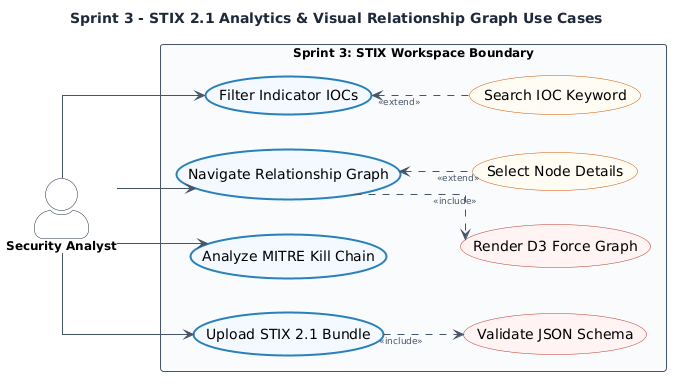
\includegraphics[width=0.95\textwidth]{assets/s3_usecase.png}
\caption{Sprint 3: Use Case diagram for the STIX 2.1 dashboard.}
\label{fig:s3_usecase}
\end{figure}

The functional workflows and validation rules for each use case are documented in Table~\ref{tab:s3_uc_desc_expanded}.

\begin{table}[H]
\centering
\small
\arrayrulecolor{charcoal!30}
\rowcolors{2}{cyberblue!5}{white}
\begin{tabularx}{\textwidth}{>{\raggedright\arraybackslash}p{2.6cm}>{\raggedright\arraybackslash}p{4.4cm}X}
\hline
\rowcolor{charcoal}
\thc{Use Case} & \thc{Actor/Trigger} & \thc{Main Workflow \& Validation Rules} \\
\hline
Upload STIX 2.1 & Security Analyst / Uploads JSON File & 1. Analyst uploads a STIX JSON file. \\
 & & 2. The parser validates the existence of the `type: "bundle"` attribute and reads the JSON structures. \\
 & & 3. If validation fails, an error toast is displayed. \\
\hline
Filter IOCs & Security Analyst / Types in Search & 1. Analyst filters by search text or select box (IP, Hash, URL). \\
 & & 2. The system executes client-side regex matching and pagination. \\
\hline
\end{tabularx}
\caption{Sprint 3: Detailed Use Case descriptions.}
\label{tab:s3_uc_desc_expanded}
\end{table}

\subsection{Sprint Conception: Parser Interfaces and Graph Sequences}

\subsubsection{STIX 2.1 Schema and Core Objects}
Standard STIX 2.1 bundles represent complex threat profiles using objects and relationships. To understand our ingestion logic, we must catalog the core STIX domain objects (SDOs) parsed by our engine, detailing their internal JSON attributes, architectural roles, and security use-cases:
\begin{itemize}
    \item \textbf{Threat Actor SDO:} Represents individuals or groups operating with malicious intent (e.g. APT29, LockBit). In the STIX 2.1 schema, this object maintains critical properties including:
    \begin{itemize}
        \item \texttt{name}, \texttt{description}, and \texttt{aliases}.
        \item \texttt{threat\_actor\_types} (e.g. \texttt{nation-state}, \texttt{spy}, or \texttt{cyber-criminal}).
        \item \texttt{roles} (e.g. \texttt{infrastructure-operator} or \texttt{malware-author}).
        \item \texttt{goals} (e.g. \texttt{financial-gain} or \texttt{espionage}).
        \item \texttt{sophistication} (ranking from \texttt{aspirant} to \texttt{innovator}).
        \item \texttt{resource\_level} (defining backing, such as \texttt{government} or \texttt{individual}).
    \end{itemize}
    In our system, this SDO forms the central root of threat intelligence investigation.
    \item \textbf{Campaign SDO:} Represents an organized grouping of adversarial behaviors, active intrusions, and operations targeting specific industries, geographic areas, or corporate assets over a defined timeline. Key attributes include \texttt{first\_seen}, \texttt{last\_seen}, \texttt{objective}, and \texttt{aliases}. Our parser resolves these attributes to build temporal threat timelines, tracking how adversaries alter their focus during seasonal cycles.
    \item \textbf{Intrusion Set SDO:} Represents a collection of malicious behaviors, patterns of activity, resources, and campaigns sharing distinct properties, attributable to a common adversary. Unlike campaigns, which are bounded by specific start and end dates and focused objectives, intrusion sets represent long-term threat profiles. Key parameters include \texttt{first\_seen}, \texttt{last\_seen}, \texttt{goals}, \texttt{secondary\_adversaries}, and standard STIX identifiers.
    \item \textbf{Malware SDO:} Programmatic malicious code designed to compromise system integrity, execute unauthorized commands, or exfiltrate private data. Key properties are:
    \begin{itemize}
        \item \texttt{malware\_types} (e.g. \texttt{trojan}, \texttt{ransomware}, \texttt{wiper}, \texttt{keylogger}).
        \item \texttt{capabilities} (e.g. \texttt{anti-debug}, \texttt{sandbox-aware}, \texttt{data-exfil}).
        \item Operating system compatibility parameters.
    \end{itemize}
    \item \textbf{Tool SDO:} Legitimate software leveraged by threat actors to perform unauthorized or malicious actions (e.g. PowerShell, Mimikatz, Cobalt Strike, Nmap). It is crucial to distinguish this from the Malware SDO, as Tools are dual-use software that standard security configurations might otherwise whitelist.
    \item \textbf{Attack Pattern SDO:} Detailed descriptions of adversary techniques, mapped to the MITRE ATT\&CK Kill Chain taxonomy. Key fields include \texttt{kill\_chain\_phases} (identifying the active stage, such as \texttt{initial-access} or \texttt{credential-access}) and \texttt{external\_references} containing MITRE ID tags (e.g., \texttt{T1190} for exploit public-facing applications).
    \item \textbf{Identity SDO:} Represents actual target victims, organizations, sectors, or individuals. Key properties are:
    \begin{itemize}
        \item \texttt{identity\_class} (e.g. \texttt{organization}, \texttt{individual}, \texttt{class}).
        \item \texttt{sectors} (\texttt{healthcare}, \texttt{finance}, \texttt{defense}).
        \item \texttt{contact\_information}.
    \end{itemize}
    \item \textbf{Indicator SDO:} Technical patterns matching observable indicators of compromise (IOCs) such as SHA-256 hashes, IP addresses, or domain links. The core attribute is \texttt{pattern}, expressed in STIX Patterning Language (e.g., \texttt{[file:hashes.'SHA-256' = '...']}), combined with \texttt{valid\_from} and \texttt{valid\_until} temporal bounds.
    \item \textbf{Relationship SRO:} Standard STIX Relationship Objects linking two SDOs via defined verbs (e.g., \texttt{threat-actor} ``uses'' \texttt{malware}, \texttt{indicator} ``indicates'' \texttt{campaign}, \texttt{malware} ``targets'' \texttt{sector}).
\end{itemize}

    To illustrate the input of our ingestion engine and demonstrate a complete, realistic intelligence structure, Table~\ref{tab:stix_bundle_objects} summarizes the STIX Domain Objects (SDOs) and Relationship Objects (SROs) parsed by our engine, with the full raw JSON bundle detailed in Appendix J.

    \begin{table}[H]
    \centering
    \small
    \arrayrulecolor{charcoal!30}
    \rowcolors{2}{cyberblue!5}{white}
    \begin{tabularx}{\textwidth}{>{\raggedright\arraybackslash}p{2.8cm}>{\raggedright\arraybackslash}p{3.6cm}X}
    \hline
    \rowcolor{charcoal}
    \thc{STIX Object Type} & \thc{Name / Identifier} & \thc{Key Characteristics / Attributes} \\
    \hline
    \texttt{threat-actor}   & Apex Spyder              & Nation-state actor, Espionage goals, Innovator sophistication \\
    \texttt{campaign}       & Operation Silent Breach  & Target: telecommunication networks tap \\
    \texttt{malware}        & SpectreShell             & Remote access trojan, DNS exfiltration, registry persistence \\
    \texttt{tool}           & SharpDump                & C\# credential exploitation (LSASS memory dumper) \\
    \texttt{attack-pattern} & LSASS Memory Dumping     & Maps to MITRE ATT\&CK phase: \texttt{credential-access} \\
    \texttt{identity}       & TelcoGlobal Inc.         & Target identity: telecommunications and technology sectors \\
    \texttt{indicator}      & SpectreShell C2 Beacon   & Pattern: \texttt{[domain-name:value = 'c2.corp-updates.net']} \\
    \texttt{relationship}   & attributed-to            & Connects campaign to threat-actor \\
    \texttt{relationship}   & uses                     & Connects threat-actor to malware, and malware to tool \\
    \texttt{relationship}   & targets                  & Connects malware and campaign to victim identity \\
    \texttt{relationship}   & indicates                & Connects indicator to malware \\
    \hline
    \end{tabularx}
    \caption{STIX 2.1 Sample Intelligence Bundle Components.}
    \label{tab:stix_bundle_objects}
    \end{table}


\subsubsection{UML Class Diagram}
The structural layout of our client-side parser services, data models, and visualization pages is illustrated in Figure~\ref{fig:s3_class}.

\begin{figure}[H]
\centering
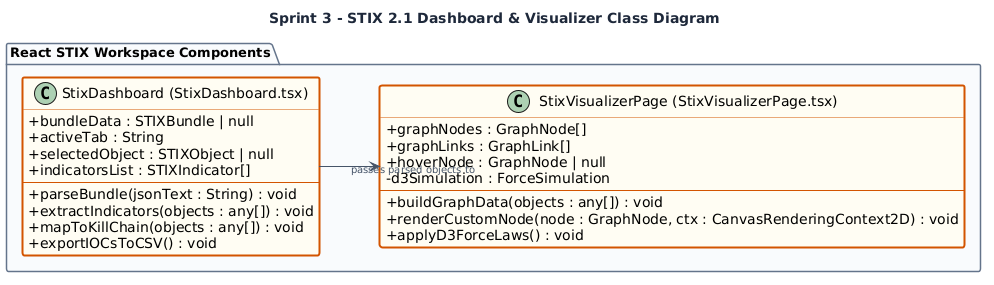
\includegraphics[width=0.95\textwidth]{assets/s3_class.png}
\caption{Sprint 3: Conception Class diagram.}
\label{fig:s3_class}
\end{figure}

\subsubsection{UML Sequence Diagram}
The asynchronous parsing and graph building lifecycle triggered when an investigator uploads a threat bundle is traced in Figure~\ref{fig:s3_sequence}.

\begin{figure}[H]
\centering
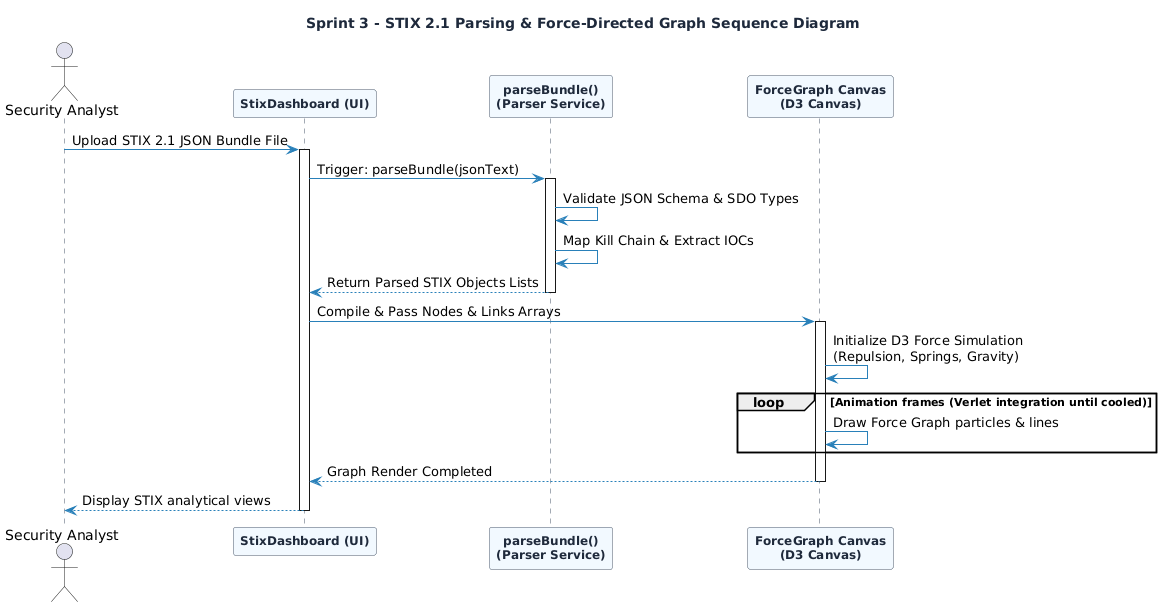
\includegraphics[width=0.95\textwidth]{assets/s3_sequence.png}
\caption{Sprint 3: Sequence diagram of STIX bundle parsing and graph rendering.}
\label{fig:s3_sequence}
\end{figure}



\subsection{Sprint Realization: STIX Ingestion and Mapping}

\subsubsection{STIX 2.1 Parser Code Walkthrough}
The parser located in `ui/StixDashboard.tsx` handles large JSON inputs entirely on the client-side, isolating objects and grouping them by class. Table~\ref{tab:stix_parser_rules} details the client-side parsing rules, sorting STIX objects by type and mapping Indicators to classes using regular expressions (with the complete parser utilities detailed in Appendix M).

    \begin{table}[H]
    \centering
    \small
    \arrayrulecolor{charcoal!30}
    \rowcolors{2}{cyberblue!5}{white}
    \begin{tabularx}{\textwidth}{>{\raggedright\arraybackslash}p{3.5cm}>{\raggedright\arraybackslash}p{4.0cm}X}
    \hline
    \rowcolor{charcoal}
    \thc{Target Object / Class} & \thc{STIX Type / Pattern Match} & \thc{Parser Mapping \& Actions} \\
    \hline
    Threat Actor   & \texttt{threat-actor}                        & Populates the actor analysis cards \\
    Malware / Tool & \texttt{malware} / \texttt{tool}              & Populates the active adversary tools inventory \\
    Attack Pattern & \texttt{attack-pattern}                      & Compiled to MITRE ATT\&CK phase matrix \\
    IPv4 Indicator & \texttt{/ipv4-addr:value/}                   & Classified as 'IPv4 Address' IOC \\
    SHA-256 Hash   & \texttt{/file:hashes\textbackslash.\allowbreak'SHA-256'/} & Classified as 'SHA-256 Hash' IOC \\
    Domain Name    & \texttt{/domain-name:value/}                 & Classified as 'Domain Name' IOC \\
    URL Endpoint   & \texttt{/url:value/}                         & Classified as 'URL Endpoint' IOC \\
    \hline
    \end{tabularx}
    \caption{STIX 2.1 Parser Object Classification Rules.}
    \label{tab:stix_parser_rules}
    \end{table}

    The parser loops through each attack pattern's \texttt{kill\_chain\_phases} array, filters for \texttt{kill\_chain\_name: "mitre-attack"}, replaces dashes with spaces for clean labels, and inserts the pattern object into a map grouped by phase name (detailed in Appendix M.1).



\section{Sprint 4: Analytics, History, and Performance Polishing}

\subsection{Sprint Backlog and Objectives}
The final sprint focused on performance stabilization, database query optimizations, and historical threat telemetry analytics. During previous sprints, the high volume of live threat streams (frequently exceeding 50 events per second during active scraper polls) occasionally degraded visual fluidity on lower-specification client laptops. Furthermore, analysts required tools to query historical databases, search specific indicators, and geolocate their local networks.

The Sprint 4 backlog focused on four critical objectives:
\begin{itemize}
    \item \textbf{Paginated Database Query Browser:} An optimized Express route querying Mongoose backend collections with search tags, regex filters, and strict page limit clamps to prevent server memory exhaustion.
    \item \textbf{"Target My IP" Geolocator:} A utility on the history page that queries public IP APIs, geolocates the client coordinate points, and automatically filters threat history to logs targeting the analyst's network.
    \item \textbf{Circular Memory Buffers (RingBuffer):} A client-side memory controller that caps active threat log buffers, avoiding JavaScript garbage collection performance overhead.
    \item \textbf{Adaptive FPS Sampling Engine:} An automated quality manager that tracks browser rendering frame rates and drops incoming events dynamically to preserve UI responsiveness.
\end{itemize}

\subsection{Sprint Analysis: Use Case Modeling}
The investigator's search and performance diagnostics use cases are captured in Figure~\ref{fig:s4_usecase}.

\begin{figure}[H]
\centering
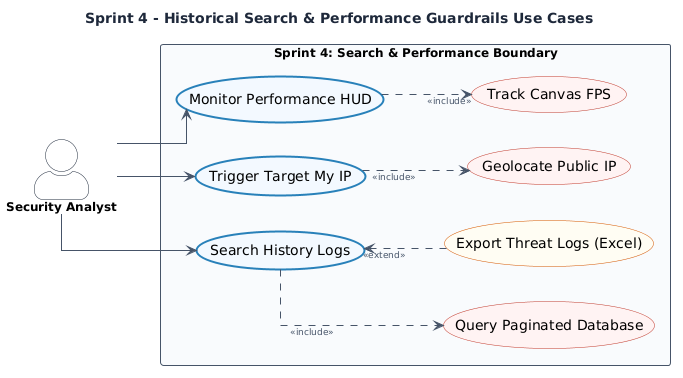
\includegraphics[width=0.95\textwidth]{assets/s4_usecase.png}
\caption{Sprint 4: Use Case diagram for database browsing and performance monitoring.}
\label{fig:s4_usecase}
\end{figure}

The functional steps are detailed in Table~\ref{tab:s4_uc_desc}.

\begin{table}[H]
\centering
\small
\arrayrulecolor{charcoal!30}
\rowcolors{2}{cyberblue!5}{white}
\begin{tabularx}{\textwidth}{>{\raggedright\arraybackslash}p{2.6cm}>{\raggedright\arraybackslash}p{4.4cm}X}
\hline
\rowcolor{charcoal}
\thc{Use Case} & \thc{Actor/Trigger} & \thc{Main Workflow} \\
\hline
Search History Logs & Security Analyst / Enters Query & The analyst submits a search. The system issues a paginated HTTP GET request to `/api/history` with query parameters. \\
Trigger Target My IP & Security Analyst / Clicks Button & Queries a public IP API (`jsonip`), geolocates the address, and immediately filters threat history to logs targeting the analyst's network. \\
Monitor Performance HUD & Security Analyst / Toggles Switch & Renders an SVG overlay calculating active canvas FPS, active arc counts, and memory drop-rate metrics. \\
\hline
\end{tabularx}
\caption{Sprint 4: Use Case descriptions.}
\label{tab:s4_uc_desc}
\end{table}

\subsection{Sprint Conception: Search and Performance Buffers}

\subsubsection{UML Class Diagram}
The structural layout of our historical logs queries, circular memory buffers, and adaptive sampling stores is illustrated in Figure~\ref{fig:s4_class}.

\begin{figure}[H]
\centering
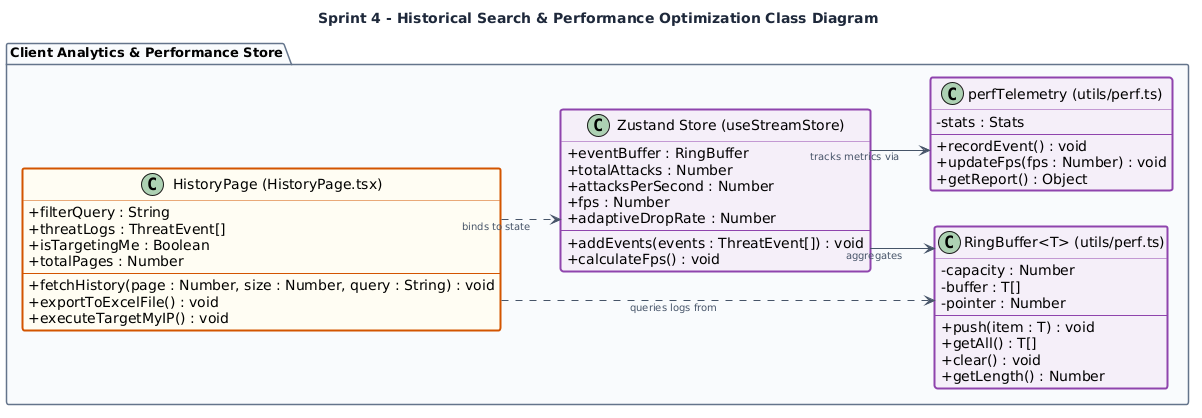
\includegraphics[width=0.95\textwidth]{assets/s4_class.png}
\caption{Sprint 4: Conception Class diagram.}
\label{fig:s4_class}
\end{figure}

\subsubsection{UML Sequence Diagram}
The paginated network round-trip tracing query submissions, backend mongoose filters, and frontend table rendering is illustrated in Figure~\ref{fig:s4_sequence}.

\begin{figure}[H]
\centering
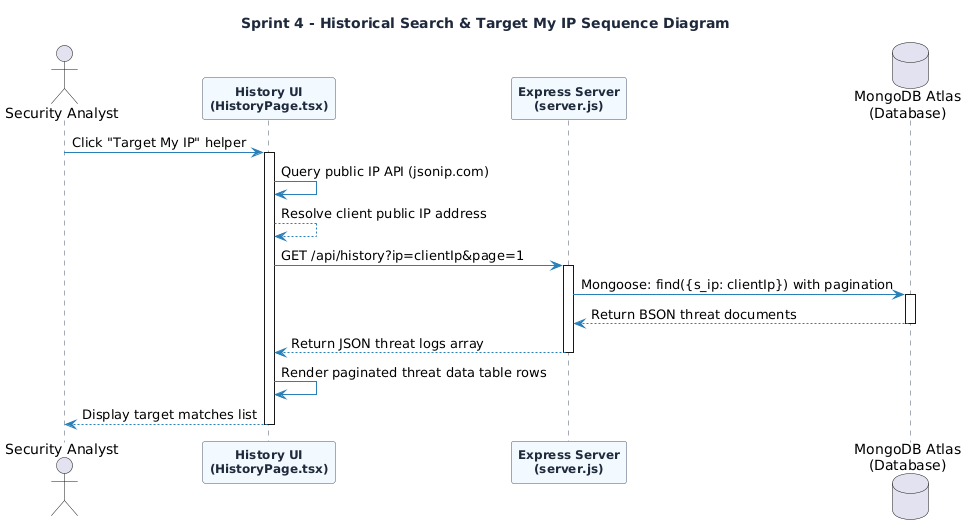
\includegraphics[width=0.95\textwidth]{assets/s4_sequence.png}
\caption{Sprint 4: Sequence diagram of paginated historical threat search.}
\label{fig:s4_sequence}
\end{figure}

\subsection{Performance Stabilization Mathematics}

\subsubsection{Garbage Collection and Memory Allocation Pressures}
In applications that process high-speed data streams, standard array operations can slow down the browser. Frequently adding and removing objects from standard arrays causes the browser to allocate and clean up memory, which can lead to frame drops and laggy visuals. To avoid this, we implemented a custom circular buffer.

\subsubsection{Circular RingBuffer Logic}
To store threat events without constantly allocating new memory, we built a circular array buffer. The buffer is initialized with a fixed capacity of 10,000 slots. As new events arrive, they are written to the next available index. When the capacity is reached, the oldest events are overwritten in-place, keeping memory usage constant and preventing performance stutters.

\subsubsection{Adaptive Event Sampling Controller}
The system monitors browser frame rates. If the rendering performance falls below specific thresholds, the ingestion engine drops a percentage of visual events to protect the interface from lagging, as defined in Table~\ref{tab:perf_drop_rules}.

\begin{table}[H]
\centering
\small
\arrayrulecolor{charcoal!30}
\rowcolors{2}{cyberblue!5}{white}
\begin{tabularx}{\textwidth}{>{\raggedright\arraybackslash}p{4.2cm}>{\raggedright\arraybackslash}p{4.2cm}X}
\hline
\rowcolor{charcoal}
\thc{Render Quality Mode} & \thc{Instant FPS Range} & \thc{Event Drop Ingestion Rate} \\
\hline
\textbf{High-Fluidity Mode} & Greater than or equal to 55 & 0\% (Processes all incoming visual events) \\
\textbf{Medium-Load Mode} & Between 30 and 55 & 50\% (Drops half of incoming visual events) \\
\textbf{Stress-Mitigation Mode} & Less than or equal to 30 & 75\% (Drops three-quarters of visual events) \\
\hline
\end{tabularx}
\caption{Adaptive Event Sampling Engine control parameters.}
\label{tab:perf_drop_rules}
\end{table}

\subsection{Sprint Realization: Performance Guardrails and Buffers}

\subsubsection{Circular Memory Buffer Implementation}
The circular buffer is coded inside `utils/perf.ts`. The complete class structure, showing its memory pre-allocation, circular writing logic, and constant-time extraction is summarized in Table~\ref{tab:ring_buffer_api}, with the complete source code detailed in Appendix K:
    
    \begin{table}[H]
    \centering
    \small
    \arrayrulecolor{charcoal!30}
    \rowcolors{2}{cyberblue!5}{white}
    \begin{tabularx}{\textwidth}{>{\raggedright\arraybackslash}p{4.0cm}>{\raggedright\arraybackslash}p{3.2cm}X}
    \hline
    \rowcolor{charcoal}
    \thc{Method / Property} & \thc{Time Complexity} & \thc{Functional Role / Behavior} \\
    \hline
    \texttt{constructor\allowbreak(capacity)} & $O(N)$ heap allocation  & Pre-allocates fixed size array to block dynamic GC triggers \\
    \texttt{push(item)}            & $O(1)$ constant time    & Overwrites index \texttt{pointer \% capacity} and increments pointer \\
    \texttt{getAll()}              & $O(N)$ linear time      & Sequentially reads elements starting from oldest index to pointer \\
    \texttt{getLength()}           & $O(1)$ constant time    & Returns the active number of records stored (capped at capacity) \\
    \hline
    \end{tabularx}
    \caption{Circular RingBuffer API Specifications.}
    \label{tab:ring_buffer_api}
    \end{table}

\subsubsection{Adaptive Event Sampling Integration}
Inside `stream/useStreamStore.ts`, the Zustand store utilizes the adaptive sampling rules. The Zustand store evaluates the current frames-per-second (`fps`) against critical performance boundaries. If the frame rate falls under 30 FPS, a drop rate of 75\% is set. If it falls under 45 FPS, a drop rate of 50\% is set. For each new streaming event, a random threshold comparison determines if Three.js WebGL arc objects should be spawned or discarded (with the complete store logic detailed in Appendix E).
By dropping only the visual vector creation and three.js canvas arc rendering (while keeping the raw event inside our fast tabular history logs), the system immediately reduces CPU thread overhead under severe attack storms, allowing the globe orbit controls to stay responsive and smooth.

\subsubsection{Browser-Side FPS Telemetry Collection Loop}
To measure frame rates, the presentation layer registers a telemetry loop using browser APIs. The loop calculates the time between frames. To prevent temporary stutters from triggering adjustments, the system calculates a smoothed average. This telemetry loop runs in the background with minimal overhead, updating the state once per second to avoid affecting rendering performance. The variables used in the collection loop are summarized in Table~\ref{tab:fps_telemetry_vars}, with the complete source code detailed in Appendix L:

    \begin{table}[H]
    \centering
    \small
    \arrayrulecolor{charcoal!30}
    \rowcolors{2}{cyberblue!5}{white}
    \begin{tabularx}{\textwidth}{>{\raggedright\arraybackslash}p{4.2cm}>{\raggedright\arraybackslash}p{3.8cm}X}
    \hline
    \rowcolor{charcoal}
    \thc{Variable / Hook} & \thc{Type / Source} & \thc{Operational Role in FPS Loop} \\
    \hline
    \texttt{setFps}               & Zustand Action Dispatcher          & Dispatches calculated frame rates to the global state store \\
    \texttt{frameCountRef}        & React \texttt{useRef<number>}      & Tracks the count of frame draws within the current second interval \\
    \texttt{lastTimeRef}          & React \texttt{useRef<number>}      & High-precision timestamp of the last second boundary \\
    \texttt{requestRef}           & React \texttt{useRef<number>}      & Reference handle of the active \texttt{requestAnimationFrame} loop \\
    \texttt{requestAnimationFrame}& Browser API                        & Coordinates paint ticks to sync calculations with refresh rate \\
    \hline
    \end{tabularx}
    \caption{FPS Telemetry Collector State Variables.}
    \label{tab:fps_telemetry_vars}
    \end{table}
By decoupling the telemetry collector hook from the main 3D rendering component and updating the Zustand state only once per second, the telemetry loop inflicts zero rendering overhead on the main JavaScript execution stack.

\section{System Project Retrospective}
With all 4 development sprints completed, we conducted a project retrospective to evaluate the Agile Scrum execution, analyze our technical achievements, and identify how key challenges were resolved.

\subsection{Scrum Development Analytics}
The project execution was highly structured, maintaining steady progress across the 12-week schedule. By keeping our Sprint Planning sessions focused, committing to realistic backlogs, and conducting daily standups, we succeeded in delivering all committed features on schedule:
\begin{itemize}
    \item \textbf{Velocity Consistency:} We estimated user stories using standard Planning Poker. The developer team maintained a stable velocity of approximately 25-30 story points per sprint, indicating highly predictable progress.
    \item \textbf{Increment Readiness:} Each sprint review concluded with a fully demonstrable software build. The Product Owner was able to interact with the scrapers in Sprint 1, rotate the 3D globe in Sprint 2, upload STIX files in Sprint 3, and test performance HUDs in Sprint 4.
\end{itemize}

\subsection{Overcoming Critical Technical Challenges}
During realization, our engineering team resolved three major technical bottlenecks:

\subsubsection{1. Visual Interface Lag}
Under heavy data loads, drawing every threat arc caused performance degradation.
\begin{itemize}
    \item \textbf{Resolution:} We implemented a 300ms event grouping queue on the server, delayed state updates, and capped active visual arcs to 150. Combined with adaptive sampling, this restored smooth performance.
\end{itemize}

\subsubsection{2. Database Storage Limits}
Continuous ingestion threatened to exceed storage limits quickly.
\begin{itemize}
    \item \textbf{Resolution:} We optimized the database schema to use compact field names, reducing storage size by 50%. We also configured automatic expiration rules for historical records and a backup monitor to halt writes if storage limits are reached.
\end{itemize}

\subsubsection{3. Resource Sharing (CORS) Blocks}
Deploying our React frontend application while running our API backend on a separate instance initially resulted in resource sharing blocks.
\begin{itemize}
    \item \textbf{Resolution:} We resolved this by configuring proxy routing rules in Vercel to direct frontend requests through internal paths, avoiding resource sharing blocks.
\end{itemize}

\subsection{Architectural Scalability and Future Improvements}
To transition the Predictra Threat Map from a prototype into an enterprise platform, the system architecture must be designed to scale horizontally. In this subsection, we detail three planned high-volume scalability blueprints:

\subsubsection{1. Kafka Distributed Message Broker Ingestion}
To prevent data loss if the backend server crashes under heavy load, we propose using a message broker like Apache Kafka. Scrapers will publish threat payloads to message queues, and the server will read and stream them to clients. This ensures a durable and fault-tolerant ingestion tier capable of handling massive threat volumes.

\subsubsection{2. Predictive Machine Learning Extensions}
A planned extension is the integration of a predictive machine learning model to anticipate threat trends. By training a model on historical threat distributions, the system can analyze patterns to forecast attack spikes and target sectors, displaying these predictions on the 3D globe as threat heatmaps.

\subsubsection{3. Sharded Geographical Database Clustering}
As historical records accumulate, a single database instance may face bottlenecks. We propose a database sharding strategy based on geographic regions. This guarantees that queries for specific countries are routed only to their corresponding database segments, minimizing search latency and scaling storage capacity.

\section{Conclusion}
This chapter detailed the completion of our second main release. By parsing STIX 2.1 JSON files client-side, mapping threat actions to MITRE ATT\&CK matrices, setting up paginated history browsers, geolocating public network IPs, and establishing performance stabilizers (including circular RingBuffers and adaptive event sampling drop rates), we have realized a highly performant, standard-compliant, and operationally reliable Cyber Threat Intelligence platform. We proceed to the General Conclusion to summarize our academic achievements, review our project goals, and suggest future avenues for research.
